\documentclass{standalone}
\usepackage{tikz}
\usetikzlibrary{patterns, positioning}

\begin{document}
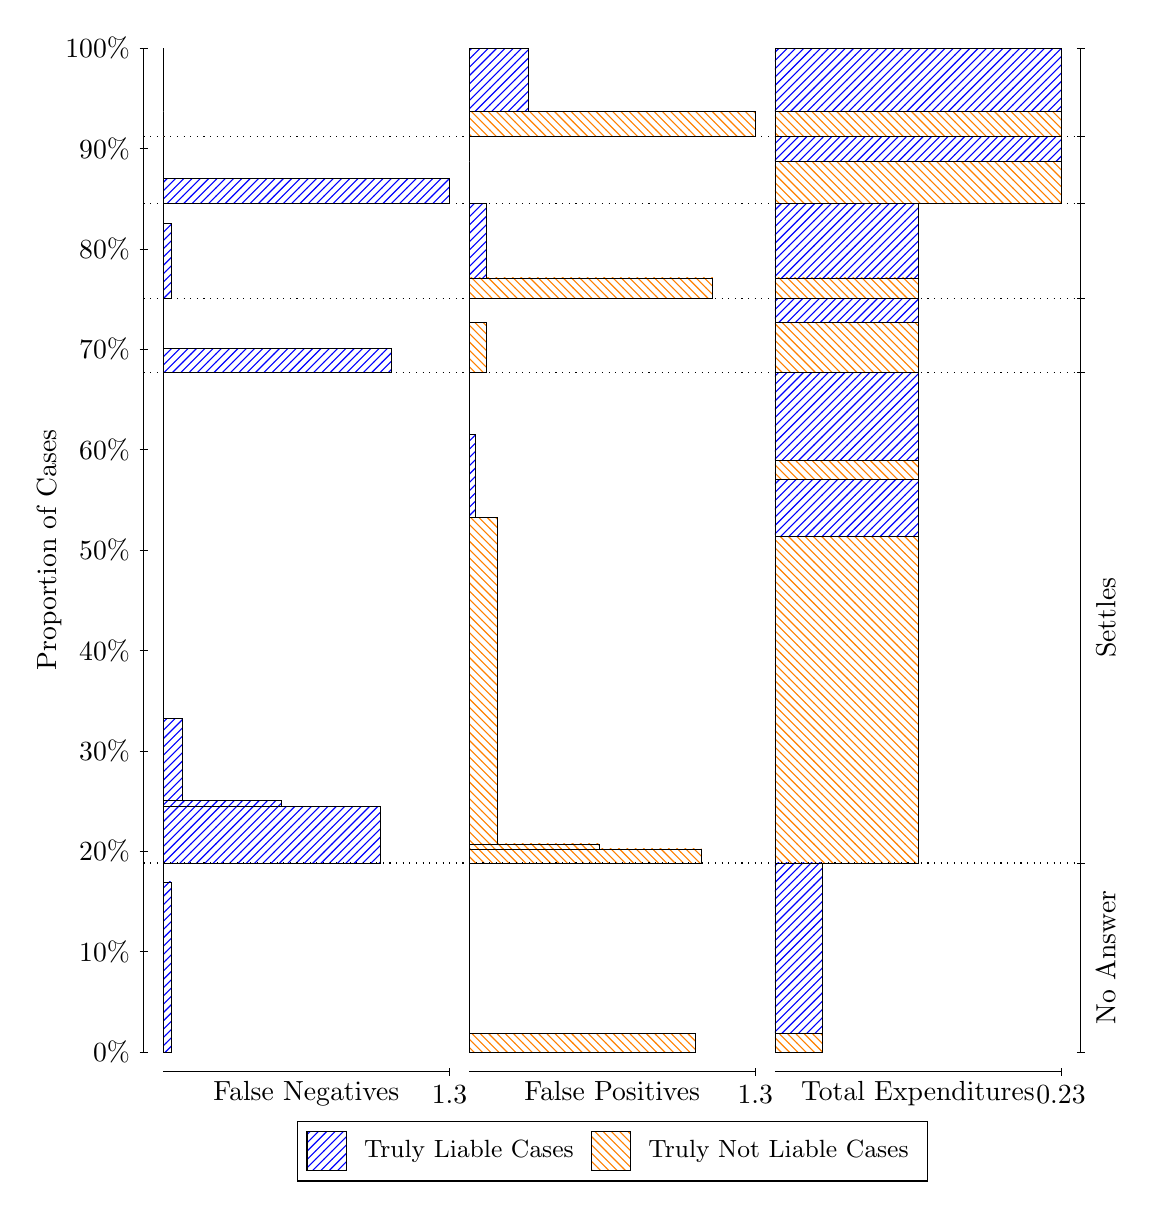
\begin{tikzpicture}
\draw[black, very thin] (1.5,1.75) -- (1.5,14.5);
\node[rotate=90, anchor=center] at (0.3, 8.125) {Proportion of Cases};
\draw[black, very thin] (1.45,1.75) -- (1.55,1.75);
\node[anchor=east] at (1.45, 1.75) {0\%};
\draw[black, very thin] (1.45,3.025) -- (1.55,3.025);
\node[anchor=east] at (1.45, 3.025) {10\%};
\draw[black, very thin] (1.45,4.3) -- (1.55,4.3);
\node[anchor=east] at (1.45, 4.3) {20\%};
\draw[black, very thin] (1.45,5.575) -- (1.55,5.575);
\node[anchor=east] at (1.45, 5.575) {30\%};
\draw[black, very thin] (1.45,6.85) -- (1.55,6.85);
\node[anchor=east] at (1.45, 6.85) {40\%};
\draw[black, very thin] (1.45,8.125) -- (1.55,8.125);
\node[anchor=east] at (1.45, 8.125) {50\%};
\draw[black, very thin] (1.45,9.4) -- (1.55,9.4);
\node[anchor=east] at (1.45, 9.4) {60\%};
\draw[black, very thin] (1.45,10.675) -- (1.55,10.675);
\node[anchor=east] at (1.45, 10.675) {70\%};
\draw[black, very thin] (1.45,11.95) -- (1.55,11.95);
\node[anchor=east] at (1.45, 11.95) {80\%};
\draw[black, very thin] (1.45,13.225) -- (1.55,13.225);
\node[anchor=east] at (1.45, 13.225) {90\%};
\draw[black, very thin] (1.45,14.5) -- (1.55,14.5);
\node[anchor=east] at (1.45, 14.5) {100\%};

\draw[black, very thin] (13.4,1.75) -- (13.4,14.5);
\draw[black, very thin] (13.35,1.75) -- (13.45,1.75);
\node[anchor=west] at (13.35, 1.75) {};
\draw[black, very thin] (13.35,4.1506) -- (13.45,4.1506);
\node[anchor=west] at (13.35, 4.1506) {};
\draw[black, very thin] (13.35,10.382) -- (13.45,10.382);
\node[anchor=west] at (13.35, 10.382) {};
\draw[black, very thin] (13.35,11.321) -- (13.45,11.321);
\node[anchor=west] at (13.35, 11.321) {};
\draw[black, very thin] (13.35,12.529) -- (13.45,12.529);
\node[anchor=west] at (13.35, 12.529) {};
\draw[black, very thin] (13.35,13.379) -- (13.45,13.379);
\node[anchor=west] at (13.35, 13.379) {};
\draw[black, very thin] (13.35,14.5) -- (13.45,14.5);
\node[anchor=west] at (13.35, 14.5) {};

\draw[black, very thin, pattern color=blue, pattern=north east lines] (1.75,1.75) rectangle (1.8548,3.9095);
\draw[black, very thin, pattern color=orange, pattern=north west lines] (1.75,3.9095) rectangle (1.75,4.1506);
\draw[black, very thin, pattern color=blue, pattern=north east lines] (1.75,4.1506) rectangle (4.5099,4.8716);
\draw[black, very thin, pattern color=blue, pattern=north east lines] (1.75,4.8716) rectangle (3.2522,4.9431);
\draw[black, very thin, pattern color=blue, pattern=north east lines] (1.75,4.9431) rectangle (1.9946,5.9893);
\draw[black, very thin, pattern color=orange, pattern=north west lines] (1.75,5.9893) rectangle (1.75,10.382);
\draw[black, very thin, pattern color=blue, pattern=north east lines] (1.75,10.382) rectangle (4.6497,10.688);
\draw[black, very thin, pattern color=orange, pattern=north west lines] (1.75,10.688) rectangle (1.75,11.321);
\draw[black, very thin, pattern color=blue, pattern=north east lines] (1.75,11.321) rectangle (1.8548,12.27);
\draw[black, very thin, pattern color=orange, pattern=north west lines] (1.75,12.27) rectangle (1.75,12.529);
\draw[black, very thin, pattern color=blue, pattern=north east lines] (1.75,12.529) rectangle (5.3833,12.846);
\draw[black, very thin, pattern color=orange, pattern=north west lines] (1.75,12.846) rectangle (1.75,13.379);
\draw[black, very thin, pattern color=orange, pattern=north west lines] (1.75,13.379) rectangle (1.75,13.696);
\draw[black, very thin, pattern color=blue, pattern=north east lines] (1.75,13.696) rectangle (1.75,14.5);
\draw[black, very thin, pattern color=orange, pattern=north west lines] (5.6333,1.75) rectangle (8.5112,1.991);
\draw[black, very thin, pattern color=blue, pattern=north east lines] (5.6333,1.991) rectangle (5.6333,4.1506);
\draw[black, very thin, pattern color=orange, pattern=north west lines] (5.6333,4.1506) rectangle (8.5832,4.3292);
\draw[black, very thin, pattern color=orange, pattern=north west lines] (5.6333,4.3292) rectangle (7.2881,4.394);
\draw[black, very thin, pattern color=orange, pattern=north west lines] (5.6333,4.394) rectangle (5.9931,8.5429);
\draw[black, very thin, pattern color=blue, pattern=north east lines] (5.6333,8.5429) rectangle (5.7053,9.589);
\draw[black, very thin, pattern color=blue, pattern=north east lines] (5.6333,9.589) rectangle (5.6333,10.382);
\draw[black, very thin, pattern color=orange, pattern=north west lines] (5.6333,10.382) rectangle (5.8492,11.015);
\draw[black, very thin, pattern color=blue, pattern=north east lines] (5.6333,11.015) rectangle (5.6333,11.321);
\draw[black, very thin, pattern color=orange, pattern=north west lines] (5.6333,11.321) rectangle (8.7271,11.58);
\draw[black, very thin, pattern color=blue, pattern=north east lines] (5.6333,11.58) rectangle (5.8492,12.529);
\draw[black, very thin, pattern color=orange, pattern=north west lines] (5.6333,12.529) rectangle (5.6333,13.062);
\draw[black, very thin, pattern color=blue, pattern=north east lines] (5.6333,13.062) rectangle (5.6333,13.379);
\draw[black, very thin, pattern color=orange, pattern=north west lines] (5.6333,13.379) rectangle (9.2667,13.696);
\draw[black, very thin, pattern color=blue, pattern=north east lines] (5.6333,13.696) rectangle (6.3888,14.5);
\draw[black, very thin, pattern color=orange, pattern=north west lines] (9.5167,1.75) rectangle (10.122,1.991);
\draw[black, very thin, pattern color=blue, pattern=north east lines] (9.5167,1.991) rectangle (10.122,4.1506);
\draw[black, very thin, pattern color=orange, pattern=north west lines] (9.5167,4.1506) rectangle (11.333,8.2994);
\draw[black, very thin, pattern color=blue, pattern=north east lines] (9.5167,8.2994) rectangle (11.333,9.0205);
\draw[black, very thin, pattern color=orange, pattern=north west lines] (9.5167,9.0205) rectangle (11.333,9.2639);
\draw[black, very thin, pattern color=blue, pattern=north east lines] (9.5167,9.2639) rectangle (11.333,10.382);
\draw[black, very thin, pattern color=orange, pattern=north west lines] (9.5167,10.382) rectangle (11.333,11.015);
\draw[black, very thin, pattern color=blue, pattern=north east lines] (9.5167,11.015) rectangle (11.333,11.321);
\draw[black, very thin, pattern color=orange, pattern=north west lines] (9.5167,11.321) rectangle (11.333,11.58);
\draw[black, very thin, pattern color=blue, pattern=north east lines] (9.5167,11.58) rectangle (11.333,12.529);
\draw[black, very thin, pattern color=orange, pattern=north west lines] (9.5167,12.529) rectangle (13.15,13.062);
\draw[black, very thin, pattern color=blue, pattern=north east lines] (9.5167,13.062) rectangle (13.15,13.379);
\draw[black, very thin, pattern color=orange, pattern=north west lines] (9.5167,13.379) rectangle (13.15,13.696);
\draw[black, very thin, pattern color=blue, pattern=north east lines] (9.5167,13.696) rectangle (13.15,14.5);
\draw[black, dotted] (1.5,4.1506) -- (13.4,4.1506);
\draw[black, dotted] (1.5,10.382) -- (13.4,10.382);
\draw[black, dotted] (1.5,11.321) -- (13.4,11.321);
\draw[black, dotted] (1.5,12.529) -- (13.4,12.529);
\draw[black, dotted] (1.5,13.379) -- (13.4,13.379);
\draw[black, very thin] (1.75,1.5) -- (5.3833,1.5);
\node[anchor=north] at (3.5667, 1.5) {False Negatives};
\draw[black, very thin] (5.3833,1.45) -- (5.3833,1.55);
\node[anchor=north] at (5.3833, 1.45) {1.3};

\draw[black, very thin] (5.6333,1.5) -- (9.2667,1.5);
\node[anchor=north] at (7.45, 1.5) {False Positives};
\draw[black, very thin] (9.2667,1.45) -- (9.2667,1.55);
\node[anchor=north] at (9.2667, 1.45) {1.3};

\draw[black, very thin] (9.5167,1.5) -- (13.15,1.5);
\node[anchor=north] at (11.333, 1.5) {Total Expenditures};
\draw[black, very thin] (13.15,1.45) -- (13.15,1.55);
\node[anchor=north] at (13.15, 1.45) {0.23};

\node[black, centered, rotate=90] at (13.72, 2.9503) {No Answer};
\node[black, centered, rotate=90] at (13.72, 7.2661) {Settles};





\draw (7.449999999999999,1.5) node[draw=none] (baseCoordinate) {};
\begin{scope}[align=center]
        \matrix[scale=0.5, draw=black, below=0.5cm of baseCoordinate, nodes={draw}, column sep=0.1cm]{
            \node[rectangle, draw, minimum width=0.5cm, minimum height=0.5cm, pattern=north east lines, pattern color=blue] {}; &
            \node[draw=none, font=\small] (B) {Truly Liable Cases}; &
            \node[rectangle, draw, minimum width=0.5cm, minimum height=0.5cm, pattern=north west lines, pattern color=orange] {}; &
            \node[draw=none, font=\small] (B) {Truly Not Liable Cases}; \\
            };
\end{scope}

\end{tikzpicture}
\end{document}